%!TEX root = ../../../main.tex
\section{Sensors and data processing} % (fold)
\label{sec:mr_sensors_and_data_processing}
In the section \ref{sec:mr_hardware} the different sensors of the robot were explained.
In this section, the information gathered by these sensors and their processing is explained.
Six different kind of sensors have been used in order to fulfil the requirements of the project.
These are:
\begin{enumerate}
	\item The camera, explained in \emph{camera processing} (\ref{sub:mr_camera_processing}) to follow the line and detect QR codes.
	\item LIDAR (\ref{sub:mr_lidar_processing}) used to map the area, to localize the robot when in free navigation (see section \ref{sub:mr_free_navigation}), to detect obstacles in front of the robot and as a skill (see section \ref{sub:skills}) to allow the robot to approach a static object.
	\item Encoders in the motors, used for the combined odometry implemented in frobomind.
	\item IMU, used in combination with the wheels odometry to know the position of the robot.
	\item Board of buttons, that equipped with two buttons and one RDG led, allows the user the start or stops the robot at the same time that indicates what is is doing with the led.
\end{enumerate}
In the following subsections the data processing made with each of the sensors is explained.

	\subsection{Camera processing} % (fold)
	\label{sub:mr_camera_processing}
	In order to move around the robot workcells, a black line has been installed in the floor so it can be tracked.
	This line communicates the workcells themselves along with the internal parts of them. 
	These are: the entrance of the workcell, the conveyor and the position where the robot must place the processed order.
	To distinguish the areas QR codes have been placed in the floor following the convention that all the groups have agreed.

	Then, the camera sensor is used with two purposes:
	\begin{itemize}
		\item Detect the line
		\item Detect and read QR codes
	\end{itemize}

	\subsubsection{Line detection} % (fold)
	\label{ssub:line_detection}
	Speed and robustness have been the priority when designing the line detection.
	The filter works at 30 FPS and with a extremely low failure rate.
	However, an inertia in the filter has also been added, so the last detected point will be returned during a certain time in case the line has been stopped being detected.

	Due to the line follower adjusting the PID given a reference point, the full image doesn't need to be interpreted.
	Because the reference point is going to be the center of the image (read section \ref{sub:mr_line_navigation}), the image is cropped with a vertical offset about the reference point.
	The width of the image is not cropped so the horizontal deviation can be measured in the largest range possible.
	After this crop, the image is binarized with an RGB threshold which give a robust detection of the black line.
	The line is then searched with a virtual horizontal line over the reference point.
	This line will cross with the black line giving two intersection points that, averaged, give the center of the line.

	In order to increase the robustness 10 equally spaced vertical lines are used. 
	The process is the same for them and the final point is the averaged one from the intersection points that are closer to themselves.
	This is done due to some noise can appear in the image (see figure \ref{fig:mr_camera_processing_2}) or a crossing line can be given (see figure \ref{fig:mr_camera_processing_3}).
	The 10 parallel lines reduces the failure rate and makes the filter very robust and fast.
	A clear representation is shown in the figure \ref{fig:mr_camera_processing_1}.
	The implementation has been carried out using the OpenCV libraries \cite{opencv}.
	
		\begin{figure}
	        \centering
	        \begin{subfigure}[H]{0.296\textwidth}
	            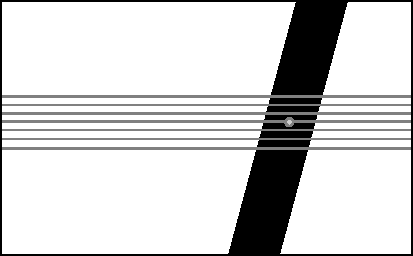
\includegraphics[width=\textwidth]{figs/mr_camera_processing_1}
	            \caption{Clear detection of the line}
	            \label{fig:mr_camera_processing_1}
	        \end{subfigure}
	        \hspace{20pt}
	        \begin{subfigure}[H]{0.296\textwidth}
	            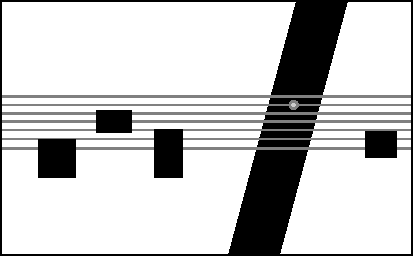
\includegraphics[width=\textwidth]{figs/mr_camera_processing_2}
	            \caption{Detection when noise in image}
	            \label{fig:mr_camera_processing_2}
	    	\end{subfigure}
	        \hspace{20pt}
	    	\begin{subfigure}[H]{0.296\textwidth}
	            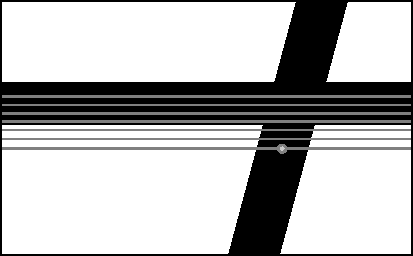
\includegraphics[width=\textwidth]{figs/mr_camera_processing_3}
	            \caption{Detection when crossing line}
	            \label{fig:mr_camera_processing_3}
	    	\end{subfigure}
	    \caption{Representation of possible cases when detecting the line}
	    \end{figure}
	% subsubsection line_detection (end)

	\subsubsection{QR detection and read} % (fold)
	\label{ssub:qr_detection_and_read}
	Due to the QR detection being done while moving, the image suffers from blur.
	This could be reduced by a Wiener motion noise filter but this is computationally expensive, so another approach has been taken.
	Instead, with inspiration from other class mates a fast shape detection is used. The shape detector looks for a white contour in the image which encapsulates a number of black elements. If a QR shape is detected, the speed is reduced until the blur no longer affects the QR reading.

	The QR detection is made using the Zlib libraries \cite{zlib}. 
	This gives the ability of easily reading the information contained in a QR code.
	% subsubsection qr_detection_and_read (end)


	% subsection camera_processing (end)

	\subsection{LIDAR processing} % (fold)
	\label{sub:mr_lidar_processing}
	The provided LIDAR (SICK TiM310) is capable of measuring the distance in 270 degrees, however due to the setup on the robot, only about 200 degrees are used. The SICK TiM Ros Package \cite{sick_tim} allows for direct set-up of minimum and maximum angles and publishes the measured points as a LaserScan message. This message then is directly used by the various skills.
	% subsection lidar_processing (end)

	\subsection{Combined frobit odometry} % (fold)
	\label{sub:mr_combined_frobit_odometry}
	The Frobit odometry module publishes the odometry status of the robot based on inputs from the wheel encoders and the on-board IMU. Sensor fusion is used to get the orientation of the robot using the IMU and this data is compared to the encoder feedback from the wheels resulting in robust odometry data.
	
	% subsection combined_frobit_odometry (end)

	\subsection{Button-board} % (fold)
	\label{sub:mr_buttons_board}
	A Tiva TM4C123 Microcontroller board is used for direct hardware control and feedback. Two buttons and a RGB led provides the hardware interface. A serial UART line connects the board to the PC.
	% subsection botton_board (end)

% section sensors_and_data_processing (end)